\documentclass[acmsmall]{acmart}
\usepackage{natbib}
\usepackage[utf8]{inputenc}
\usepackage{todonotes}
\usepackage{listings}
\usepackage{color}
\usepackage{hyperref}   
\usepackage{semantic}
\usepackage{wrapfig}
\usepackage{tikz}
\reservestyle{\keyword}{\texttt}
\keyword{match,with}
\reservestyle{\mathvar}{\textrm}
\keyword{pattern,body}
\hypersetup{
    colorlinks=true,
    linkcolor=blue,
    filecolor=red,      
    urlcolor=magenta,
    breaklinks=true,            
}
\usepackage{breakurl}  
\usepackage{pifont}% http://ctan.org/pkg/pifont
\newcommand{\cmark}{\ding{51}}%
\newcommand{\xmark}{\ding{55}}%
\newcommand{\early}{blue}
\newcommand{\express}{olive}
\newcommand{\reach}{red}

\renewcommand\todo[1]{\textcolor{orange}{#1}}

\lstset{mathescape=true,
        literate=
               {->}{$\rightarrow{}$}{1},
        morekeywords={if,then,else,return, match, with},
        basicstyle=\ttfamily,
        tabsize=2
        }

\title{A Survey of Pattern Matching in General Purpose Programming Languages}

\author{Matthew Roberts}
\email{matthew.roberts@mq.edu.au}
\orcid{0000-0002-2553-6157}
\affiliation{%
  \institution{Macquarie University}
  \city{Sydney}
  \country{Australia}
}

\acmBooktitle{Computing Surveys}

\begin{document}

\begin{abstract}
We survey existing pattern matching mechanisms in general purpose programming languages.  We describe pattern matching in popular and influential languages.  We develop and describe a lose lattice of pattern matching \emph{classes} which are ordered by expressiveness.  For each class we provide a precise definition, characterise the expressiveness, discuss existing instances from general purpose programming languages, give examples from open-source code in multiple languages, and discuss implementation options.  We also provide an historical perspective, highlighting important advances in the development of pattern matching and point to domain specific languages where their implementations of pattern matching are instructive
\end{abstract}

\maketitle

\section{Introduction}

\emph{Pattern Matching} is a control-flow mechanism available in many programming languages. There are a wide variety of implementations and design choices, but no comprehensive discussion of the differences between these.  There is also no universally agreed definition of "pattern matching". 

\subsection{Audience}
The authors of this work have two primary audiences in mind.  

\emph{Programming language designers} will be interested to see, in one place, a full map of alternative pattern matching forms.  They will have easy access to a clear and precise description of what is gained by incorporating new features, as well as guidance for implementing those features themselves.  

\emph{Developers} will be interested to see a precise definition of the forms of pattern matching they use in their own programs.  These will allow them to see ways to incorporate pattern-styles of programming even if the language does not support it and will show them the landscape in which their own work fits.  It will inform developers deciding which language to use when starting new projects.  

We also hope this work will also inform discussions in the wider programming community where languages are considering adding pattern matching and that, by collecting and organising examples, we might provide some summary of the ways in which pattern matching can support certain styles of programming.

\section{History}
We now provide a timeline of important events in the development of pattern matching.  The developments can be broken into three broad phases:
\begin{itemize}
    \item early implementations,
    \item expressivity and correctness,
    \item expanding the reach,
\end{itemize}

\subsection{Early Implementations}

Pattern matching was first described by Burstall \cite{burstall_proving_1969} in the same paper where he described proofs by structural induction on programs\footnote{There is some suggestion in that paper, and in Burstall's acceptance of the SIGPLAN Programming Langauges Achievement Award\cite{wadler_sigplan_2009}, that Robin Popplestone may have had a hand in this}. Indeed, pattern matching was introduced as a way to support such proofs.  It is notable that Burstall's account is remarkably complete  and modern in its presentation.  While other early efforts seems divorced from how pattern matching has come to be used, Burstall found the \emph{right} account of it from the very start.  McBride\cite{mcbride_computer_1970} extended LISP with a pattern matching operation in 1970 to better support computer algebra.  McBride does not cite Burstall, instead drawing inspiration from SIN, a symbolic integration system from MIT in 1967.  SIN maintains a bank of possible rules to apply and recursively applies the right one based on the top level form of the term under investigation.  Thus McBride's ?? was to create an in-language, programmer-specifiable bank of rules and supply the machinery needed to control its application during program execution.  SCRATCHPAD \cite{jenks_scratchpad_1974} was another early computer algebra system which used pattern matching in a similar way to SIN and which would influence the development of HOPE.   Implementations continued in the 1970's with Turner's development of SASL \cite{turner_history_2013, turner_sasl_1976}.  From the mid-1970s control-flow based on Algebraic Data Types is a key concern, the idea of these ADTs having been introduced as early as 1966 by Landin \cite{landin_next_1966}\footnote{Landin's 1966 paper is one of the common threads, clearly having sparked a train of thought that lead inexorably towards pattern matching}.  A single-level matching feature existed in PAL \cite{evans_palx2014language_1968} and inspired Turner's multi-level version in SASL. \todo{If this is true, PAL needs to be promoted above McBride's LISP, but the documentation on PAL shows nothing I would call pattern matching, thus the more weasley word "proto" I picked up from elsewhere} In 1978, Turner \cite{turner_recursion_1978} made a compelling case for the utility of this style of programming, linking it to the "recursion equations" which are a common form for expressing recursive algorithms in mathematics.

Logic programming has a clear influence on early pattern matching formulations.  Both Prolog and OBJ are mentioned explicitly as influences on Hope \cite{burstall_hope_1980}.  We will return to the relationship between pattern matching and logic programming in section ??.   However, in practice, pattern matching at this time is focusing more and more on  deconstructing the algebraic data types.  Using the same token, delineated by context, to indicate construction \emph{and} destruction of algebraic data has become standard practice.  This treatment found particularly clear expressions in HOPE\cite{burstall_hope_1980} and Standard ML\cite{milner_proposal_1984}.  By the middle of the 1980's the utility of, and basic form of this type of programming was well-established in research and static checks such as exhaustiveness checking were present.  Hope and ML can be considered the results of these early efforts on which later efforts build.

Thus we can see that early efforts in pattern matching were a mix of influeces from \emph{logic programming}, \emph{computer algebra}, and \emph{Landin's inspiration to algebraic data types}.  However, from here we will focus on the general purpose programming languages and leave discussions of computer algebra and logic languages to their own sections.
Then followed explorations of evaluation order, and with those came lazy implementations of the same ideas \cite{augustsson_compiler_1984}.  It is at this point that the semantics of pattern matching started receiving more attention.  A particularly clear and influential treatment of pattern matching compilation was given by Augustsson during this period \cite{augustsson_compiling_1985}. \todo{get your marangret on here}

\todo{John Darlington is responsible for the equational style we see in Haskell, which came via Miranda and SASL where Turner implemented them - see the lambda days talk.  Darlington (who was a PhD student of Burstall, implemented it in his langauge NPL (which became hope) in the early 70s - find a good ref for that please}

\todo{KRC (turner) introduced guards}

\tikzset{every picture/.style={line width=0.75pt}} %set default line width to 0.75pt   
\begin{wrapfigure}{l}{0.5\textwidth}
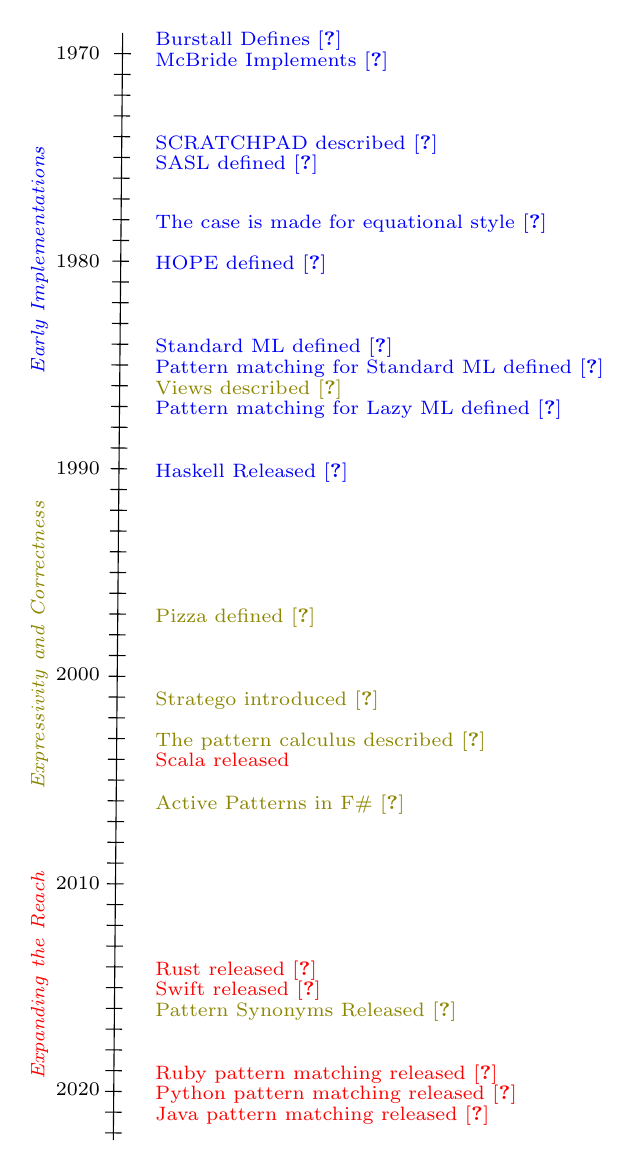
\begin{tikzpicture}[x=0.75pt,y=0.75pt,yscale=-1,xscale=1]


\draw    (35.5,2.25) -- (31,535.75) (39.41,12.28) -- (31.41,12.21)(39.32,22.28) -- (31.32,22.21)(39.24,32.28) -- (31.24,32.21)(39.15,42.28) -- (31.15,42.21)(39.06,52.28) -- (31.06,52.21)(38.97,62.28) -- (30.97,62.21)(38.89,72.28) -- (30.89,72.21)(38.8,82.28) -- (30.8,82.21)(38.71,92.28) -- (30.71,92.21)(38.62,102.28) -- (30.62,102.21)(38.54,112.28) -- (30.54,112.21)(38.45,122.28) -- (30.45,122.21)(38.36,132.28) -- (30.36,132.21)(38.27,142.28) -- (30.27,142.21)(38.19,152.28) -- (30.19,152.21)(38.1,162.28) -- (30.1,162.21)(38.01,172.28) -- (30.01,172.21)(37.92,182.28) -- (29.92,182.21)(37.83,192.28) -- (29.84,192.21)(37.75,202.28) -- (29.75,202.21)(37.66,212.28) -- (29.66,212.21)(37.57,222.28) -- (29.57,222.21)(37.48,232.28) -- (29.48,232.21)(37.4,242.28) -- (29.4,242.21)(37.31,252.28) -- (29.31,252.21)(37.22,262.28) -- (29.22,262.2)(37.13,272.27) -- (29.13,272.2)(37.05,282.27) -- (29.05,282.2)(36.96,292.27) -- (28.96,292.2)(36.87,302.27) -- (28.87,302.2)(36.78,312.27) -- (28.78,312.2)(36.7,322.27) -- (28.7,322.2)(36.61,332.27) -- (28.61,332.2)(36.52,342.27) -- (28.52,342.2)(36.43,352.27) -- (28.43,352.2)(36.35,362.27) -- (28.35,362.2)(36.26,372.27) -- (28.26,372.2)(36.17,382.27) -- (28.17,382.2)(36.08,392.27) -- (28.08,392.2)(35.99,402.27) -- (27.99,402.2)(35.91,412.27) -- (27.91,412.2)(35.82,422.27) -- (27.82,422.2)(35.73,432.27) -- (27.73,432.2)(35.64,442.27) -- (27.64,442.2)(35.56,452.27) -- (27.56,452.2)(35.47,462.27) -- (27.47,462.2)(35.38,472.27) -- (27.38,472.2)(35.29,482.27) -- (27.29,482.2)(35.21,492.27) -- (27.21,492.2)(35.12,502.27) -- (27.12,502.2)(35.03,512.27) -- (27.03,512.2)(35.03,522.27) -- (27.03,522.2)(35.03,532.27) -- (27.03,532.2) ;

% Years
\draw (2,8) node [anchor=north west][inner sep=0.75pt]  [font=\scriptsize] [align=left] {1970};
\draw (2,108) node [anchor=north west][inner sep=0.75pt]  [font=\scriptsize] [align=left] {1980};
\draw (2,207.5) node [anchor=north west][inner sep=0.75pt]  [font=\scriptsize] [align=left] {1990};
\draw (2,307) node [anchor=north west][inner sep=0.75pt]  [font=\scriptsize] [align=left] {2000};
\draw (2,407.5) node [anchor=north west][inner sep=0.75pt]  [font=\scriptsize] [align=left] {2010};
\draw (2,507) node [anchor=north west][inner sep=0.75pt]  [font=\scriptsize] [align=left] {2020};

% Events
\draw (50,0) node [anchor=north west][inner sep=0.75pt]  [font=\scriptsize, color=\early] [align=left] {Burstall Defines \cite{burstall_proving_1969}};
\draw (50,10) node [anchor=north west][inner sep=0.75pt]  [font=\scriptsize, color=\early] [align=left] {McBride Implements \cite{mcbride_computer_1970}};
\draw (50,50) node [anchor=north west][inner sep=0.75pt]  [font=\scriptsize, color=\early] [align=left] {SCRATCHPAD described \cite{jenks_scratchpad_1974}};
\draw (50,60) node [anchor=north west][inner sep=0.75pt]  [font=\scriptsize, color=\early] [align=left] {SASL defined \cite{turner_sasl_1976}};

\draw (50,88) node [anchor=north west][inner sep=0.75pt]  [font=\scriptsize, color=\early] [align=left] {The case is made for equational style \cite{turner_recursion_1978}};
\draw (50,108) node [anchor=north west][inner sep=0.75pt]  [font=\scriptsize, color=\early] [align=left] {HOPE defined \cite{burstall_hope_1980}};

\draw (50,148) node [anchor=north west][inner sep=0.75pt]  [font=\scriptsize, color=\early] [align=left] {Standard ML defined \cite{cardelli_compiling_1984}}; 
\draw (50,158) node [anchor=north west][inner sep=0.75pt]  [font=\scriptsize, color=\early] [align=left] {Pattern matching for Standard ML defined \cite{cardelli_compiling_1984}};
\draw (50,168) node [anchor=north west][inner sep=0.75pt]  [font=\scriptsize, color=\express] [align=left] {Views described \cite{}}; 
\draw (50,178) node [anchor=north west][inner sep=0.75pt]  [font=\scriptsize, color=\early] [align=left] {Pattern matching for Lazy ML defined \cite{augustsson_compiling_1985}}; 
\draw (50,208) node [anchor=north west][inner sep=0.75pt]  [font=\scriptsize, color=\early] [align=left] {Haskell Released \cite{peyton_jones_haskell98_nodate}}; 

\draw (50,278) node [anchor=north west][inner sep=0.75pt]  [font=\scriptsize, color=\express] [align=left] {Pizza defined \cite{odersky_pizza_97}}; 
\draw (50,318) node [anchor=north west][inner sep=0.75pt]  [font=\scriptsize, color=\express] [align=left] {Stratego introduced \cite{}}; 
\draw (50,338) node [anchor=north west][inner sep=0.75pt]  [font=\scriptsize, color=\express] [align=left] {The pattern calculus described \cite{jay_pattern_2004}}; 
\draw (50,348) node [anchor=north west][inner sep=0.75pt]  [font=\scriptsize, color=\reach] [align=left] {Scala released}; 
\draw (50,368) node [anchor=north west][inner sep=0.75pt]  [font=\scriptsize, color=\express] [align=left] {Active Patterns in F\# \cite{syme_extensible_2007}}; 

\draw (50,448) node [anchor=north west][inner sep=0.75pt]  [font=\scriptsize, color=\reach] [align=left] {Rust released \cite{}}; 
\draw (50,458) node [anchor=north west][inner sep=0.75pt]  [font=\scriptsize, color=\reach] [align=left] {Swift released \cite{}}; 
\draw (50,468) node [anchor=north west][inner sep=0.75pt]  [font=\scriptsize, color=\express] [align=left] {Pattern Synonyms Released \cite{pickering_pattern_2016}}; 

\draw (50,498) node [anchor=north west][inner sep=0.75pt]  [font=\scriptsize, color=\reach] [align=left] {Ruby pattern matching released \cite{ruby_ruby_2019}}; 

\draw (50,508) node [anchor=north west][inner sep=0.75pt]  [font=\scriptsize, color=\reach] [align=left] {Python pattern matching released \cite{kohn_dynamic_2020}}; 
\draw (50,518) node [anchor=north west][inner sep=0.75pt]  [font=\scriptsize, color=\reach] [align=left] {Java pattern matching released \cite{}}; 

\draw (-10,168) node [anchor=north west, rotate=90][inner sep=0.75pt]  [font=\scriptsize, color=\early] [align=left] {\emph{Early Implementations}}; 
\draw (-10,368) node [anchor=north west, rotate=90][inner sep=0.75pt]  [font=\scriptsize, color=\express] [align=left] {\emph{Expressivity and Correctness}}; 
\draw (-10,508) node [anchor=north west, rotate=90][inner sep=0.75pt]  [font=\scriptsize, color=\reach] [align=left] {\emph{Expanding the Reach}}; 

\end{tikzpicture}
\label{fig:history}
\caption{Major events in the development of pattern matching}
\end{wrapfigure}

\subsection{Expressivity and Correctness}
As pattern matching became routine in functional languages, people looked for ways to extend it and to bring it to other programming paradigms.  The fact that patterns were striclty tied to the methods of constructing data were addressed.  Proposals to allow arbitrary ways of matching on a value and deconstructing it were proposed.  Wadler's views \cite{wadler_views:_1987} were first and followed by XX XX XX.  Programmers wanting to use patterns in OO languages also realised they needed to allow the programmer to define deconstruction methods which could be employed in pattern matching.  The earliest attempts were XX and XX and XX.

Also around this time, formal accounts of pattern matching semantics and accounts of computation centered around pattern matching were published.  

\begin{itemize}
  \item First Class Patterns
  \item A calculus of patterns
  \item Object Oriented pattern matching
  \item Active Patterns/Views/Non-linearity
\end{itemize}

\subsection{Expanding the Reach}

During this period, pattern matching came to mainstream languages.  While Haskell and ML had strong communities of programmers, are used in industry, and have a fair mind-share, the vast bulk of programming is still done in other languages.  Scala's mindshare was probably responsible for spreading the desire for pattern matching, but it took until Rust and Swift were released in 2004 and 2005 for pattern matching to come to languages that would eventually become mainstream.  In 2019 pattern matching arrived in Ruby, in 2020 it was described for Python and added to python 3.10.  In 2021 Java 17 included a rudimentary but recognisable form of pattern matching.  In particular Python and Java account for a significant share of the programming language "marketplace", meaning pattern matching has truly become available in the "mainstream".

\section{Expressiveness}
\label{sec:express}
We will order our classes of pattern matching according to \emph{expressiveness}.  Comparing the expressiveness of two programming constructs is notoriously difficult.  Felleisen \cite{Felleisen91} gives a formal treatment of the expressiveness of programming languages and we will work from that starting point.  We are not comparing programming languages as a whole, we are comparing program fragments.  Conceptually, we are considering different possible pattern matching forms that might be added to a hypothetical language we never define.

Felleisen asserts that a language $L$ is more expressive than another language $L'$ if there is some expression in $L$ (and a context in which to evaluate it) that has no structurally equivalent form in $L$.

Because we are working from a hypothetical general purpose (and Turing complete) language, we adopt the following definition, based on Felleisen's.

\begin{quote}
    One pattern matching form $P$ is more expressive than another $P'$ ($P \succ P')$ if there is exists an expression in $P$ for which there is no structurally equivalent expression in $P'$ \emph{assuming the existence of conditionals \footnote{c-style \lstinline{if} and \lstinline{case} forms}, functions, looping, binding, and assignment}.
    
    \emph{Structural equivalence} is strictly a local translation where the meaning of other parts of the language don't change.
    
    We will use the symbol $\varnothing$ to represent the hypothetical language with conditions, functions, looping, binding, and assignment.
\end{quote}

I.e. If you can translate from one form to another without changing the evaluation or modifying the structure, then you have gained no expressiveness.  We assume the presence of language forms that are present in most languages so that if, for example, a pattern matching form can be reduced to some other form with the addition of an assignment statement, it is not considered an increase in expressiveness.

\subsubsection{Beyond expressiveness}
There are reasons beyond expressiveness to prefer one programming form over another; but they are subjective and dependent on the programming community of practice.  We have focussed on expressiveness but don't neglect the subject experience of programming.  For each class of patterns we will include a \emph{discussion} section where we will address the subjective arguments.  It is left to the reader to decide if a particular pattern matching form is \emph{good} or not.  We note particularly that \emph{not} changing expressiveness between classes is not reason enough to reject one class of pattern matching forms.

\subsection{Scope}
We restrict ourselves to \emph{important}, \emph{commonly used}, or \emph{representative} examples in this paper.  We will also place a significant number of popular languages into the framework, even if only to note that they don't support pattern matching.

\section{Definition}
It is not immediately obvious what we might use as an explicit definition of pattern matching. Indeed, many authors will define "patterns" but not "pattern matching".

\subsection{A first attempt}

A possible definition is 

\begin{quote}
    Pattern matching is a control-flow mechanism by which the \emph{structure} of a datum is used to choose between possible \emph{resulting computations}.
\end{quote}

i.e. it is the way we transfer meaning in data to computational outcomes.

We will use the following standard form pattern matching expressions/statements in this work

\begin{lstlisting}
match expression with 
    pattern$_i$ -> body$_i$
    ...
    pattern$_n$ -> body$_n$
\end{lstlisting}

\lstinline{expression} is evaluated to a value and that value is checked against each pattern to decide which body to execute. Full details in section \ref{sec:defn}.

You will note that the above definition includes the humble \lstinline{if} statement. A c-style \lstinline{switch} statement can similarly be encoded in this form. We will conclude that this broad definition is not appropriate, but lets first follow this line of inquiry to its conclusion by explicitly converting c-style \lstinline{if} and \lstinline{switch} into pattern matches.  Figure \ref{fig:kar_if} shows how a c-style \lstinline{if} statement would look as a pattern match and figure \ref{fig:kar_switch} shows how a c-style \lstinline{switch} would look.

\begin{figure}
\hspace{-2em}
\begin{minipage}[t]{0.35\linewidth}
\begin{lstlisting}[language=C]
if (x < v[mid])
    high = mid + 1;
else if (x  > v[mid])
    low = mid + 1;           
else  
    return mid;
\end{lstlisting}
\end{minipage}
\begin{minipage}[t]{0.65\linewidth}
\begin{lstlisting}
match (x < mid) with
    true -> high = mid + 1;
    false -> match (x > v[mid]) with
                true -> low = mid + 1;
                false -> return mid;
\end{lstlisting}
\end{minipage}
\caption{This classic example of an if-statement \cite{kernighan_c_1988} is semantically equivalent to the given pattern match.  In the case that the expression being scrutinised is \lstinline{true} then one statement is executed.  In the case that the expression}
\label{fig:kar_if}
\end{figure}

\begin{figure}
\begin{minipage}[t]{0.45\linewidth}
\begin{lstlisting}[language=C]
switch (c) {
    case '0': case '1': case '2': 
    case '3': case '4': case '5': 
    case '6': case '7': 
    case '8': case '9':
        ndigit[c-'0']++;
        break;
    case ' ': 
    case '\n': 
    case '\t':
        nwhite++;
        break;
    default:
        nother++;
        break;
}
\end{lstlisting}
\end{minipage}
\begin{minipage}[t]{0.45\linewidth}
\begin{lstlisting}
match c with
    '0'  -> ndigit[c-'0']++;
    '1'  -> ndigit[c-'0']++;
    '2'  -> ndigit[c-'0']++;
    '3'  -> ndigit[c-'0']++;
    '4'  -> ndigit[c-'0']++;
    '5'  -> ndigit[c-'0']++;
    '6'  -> ndigit[c-'0']++;
    '7'  -> ndigit[c-'0']++;
    '8'  -> ndigit[c-'0']++;
    '9'  -> ndigit[c-'0']++;
    ' '  -> nwhite++;
    '\n' -> nwhite++;
    '\t' -> nwhite++;
    x    -> nother++;
\end{lstlisting}
\end{minipage}
\caption{Converting this well known switch statement \cite{kernighan_c_1988} to a pattern match is verbose, but simple}
\label{fig:kar_switch}
\end{figure}

To support these example, we need two types of patterns:
\begin{itemize}
    \item literal patterns
    \item variable patterns
\end{itemize}

In fact, one way we distinguish the different pattern matching systems we see is by what set of patterns they admit.

To be precise, we can model if and switch-statements in c with a pattern matching mechanism that works on booleans and integers and which admits literal and wildcard patterns.

However, this is clearly too broad and not representative of what programmers think of as pattern matching. While recognising that this simpler form is in the same lineage as pattern matching, we restrict out definition a little further

\subsection{Our final definition}

\begin{quote}
     Pattern matching is a control-flow mechanism by which some structure of \emph{any expressible datum} is used to choose between possible resulting computations \emph{and} to simultaneously bind variables to (sub-)structures of that datum.
\end{quote}

We have added the requirements that the one mechanism can work for all data-types expressible in the language and that the act of choosing a branch will also bind some variables. This excludes the grand-parent forms and focuses on forms that will need some interpretation to be converted into those simpler forms. It also excludes simpler binding forms such as lambda expressions and thus, we think, represents the simplest and most meaningful definition.


\subsection{Formal Definition}
\label{sec:defn}

Pattern match constructs\footnote{A pattern match is an \lstinline{expression} if all \lstinline!body$_i$! are expressions, it is a statement if all \lstinline!body$_i$! are statements.  A pattern match cannot have a mix of statements and expressions in \lstinline!body$_i$!.}
 are of the form

\begin{lstlisting}
match expression with 
    pattern$_1$ => body$_1$
    pattern$_2$ => body$_2$
    ...
    pattern$_n$ => body$_n$
\end{lstlisting}
or, equivalently

$$
\<match>\ e\ \<with>\ (p_i => b_i)
$$


Where \lstinline{pattern$_i$} ($p_i$) can bind variables for use in \lstinline{body$_i$} ($b_i$) and where \lstinline{expression} ($e$) may take on any expression in the language.

The different possible forms of pattern matching are captured in the different forms a pattern can take.  For each form, the semantics will be defined through the pattern match relation which states that expression $e$ matches with pattern $p$, giving variable subsitutions $\sigma$ if and only if there exists a $\sigma$ such that $e = \sigma p$.  I.e. it is possible to construct a sequence of variable for expression substitutions that make the pattern equal to the subject expression.

The small-step operational semantics of pattern matching are given in figure \ref{fig:small-step}.  Since these rely on the matching relation, the semantics are only partially defined until we complete that definition.  We will provide a different matching relation for each class of pattern matching we encounter.  The semantics described in figure \ref{fig:small-step} are that: the expression being scrutinised is evaluated until it is a value and then checked against each pattern from the top of the list to the bottom until one matches.  If none match, the result of the pattern is \lstinline{nil} where \lstinline{nil} is no-op in the case of a statement pattern, or some "null" value from the language in the case of an expression pattern.  These are strict semantics and thus are certainly not applicable in lazy languages like Haskell and Clean.  In those cases, the correct semantics are more subtle, but the difference does not affect our discussion.  Please note that the formal semantics provided here aim to be explicit but not necessarily universal.  What we mean by this is that there is great value in being precise in our discussion but that the variability in the languages we look at mean there is no semantics we can give that universally applies.  The semantics given in this paper will give the reader a way to precisely differentiate various pattern matching constructs, but do not provide a way to precisely recreate any particular language.

\begin{figure}
    \[
    \inference[ESubject]
    {e\ --> e'}
    {\<match>\ e\ \<with>\ (p_i -> b_i)^{*} --> \<match>\ e'\ \<with>\ (p_i -> b_i)^{*}}\]
    \[
    \inference[EMatchSucc]
    {\exists \sigma .\quad v = \sigma p1
    }
    {\<match>\ v\ \<with>\ (p_i -> b_i)^{*} --> \sigma b_1}
    \]
    \[
    \inference[EMatchFail]
    {\not \exists \sigma . \quad v = \sigma p1
    }
    {\<match>\ v\ \<with>\ (p_i -> b_i)^{*} --> \<match>\ v\ \<with>\ (p_2 -> b_2)^{*}}
    \]
        \caption{Partially defined operational semantics of pattern matching}
        \label{fig:small-step}
\end{figure}
    
\subsection{Patterns outside pattern matching}
The most important part of a pattern matching system, and the axis on which we discriminate between them, is the patterns that can be used in discriminating between branches.  Thus, patterns themselves are interesting enough.  In some languages, patterns can exist outside a pattern matching form, most commonly in an assignment operation.

For example,
$$
\<pattern> = expr
$$
would be an assignment operation that binds variables in $\<pattern>$ to parts of the result of $expr$.  An example is Javascript's destructuring assignment, shown in figure \ref{fig:destructuring_js}.  These forms, which don't include control flow, include many of the interesting features of pattern matching and much of what we discuss here is applicable there, but we don't discuss them in detail because they don't fit in our definition.  Others have included such forms in pattern matching, but invariably take care to distinguish it from the more complete form.  Kohn et. al. call it "unconditional pattern matching" for example  \cite{Kohn20}.
\begin{figure}
    \begin{lstlisting}
    [a, b] = [10, 20];
    \end{lstlisting}
    \caption{Destructing assignment in Javascript, binding \lstinline{a} to \lstinline{10} and \lstinline{b} to \lstinline{20} via a list pattern.}
    \label{fig:destructuring_js}
\end{figure}

In languages where compile-time correctness is a high priority, the language specification will define a subset of patterns as "irrefutable" and allow these in assignment operations (like above) because the match against such a pattern can never fail and control flow considerations are thus unnecessary.  Other languages will cause run-time failure or assignment of null values in the case where the pattern match has failed.

A possible design choice, that we have seen only in Stratego, is to reify a special run-time value FAIL and to have that be the result of any failed pattern match.  Many languages use this mechanism internally, but all restrict themselves to syntactic forms that guarantee the FAIL value never leaks (such as pattern matching) or treat it a a general NULL value at runtime.  Stratego is required to reify failure because it admits \emph{first-class patterns}, which are discussed in section \ref{sec:first-class}\footnote{Stratego is not a general purpose language, it is a term-rewriting language.}.

\section{Pattern matching forms}
There are three forms in which pattern matching usually comes: dedicated match; extended switch; equational reasoning.

In functional languages such as Haskell, or functionally-influenced languages like Scala and Rust, there will be a \lstinline{match} syntax using either the \lstinline{match} or \lstinline{case} keyword (shown in Figure \ref{lst:haskell_rust}).  In such languages, the right-hand side of a case is invariably an expression and the result of the whole pattern match is the result of whichever case was run.

\begin{figure}
\hspace{-2em}
\begin{minipage}[t]{0.35\linewidth}
\begin{lstlisting}
factorial n = case n of
  0 => 1
  x => x*factorial(x-1)    
\end{lstlisting}
\end{minipage}\hspace{2em}
\begin{minipage}[t]{0.55\linewidth}
\begin{lstlisting}
fn factorial(n : i32) -> i32{
    match n {
        0 => return 1,
        x => return factorial(x-1)*x
    }
}
\end{lstlisting}
\end{minipage}
\caption{Factorial in Haskell (left) and Rust (right).}
\label{lst:haskell_rust}
\end{figure}

In imperative languages like Ruby and Swift, the switch statement is often extended to support binding (shown in Figure \ref{lst:ruby_swift}).  These forms may still require the \lstinline{break} statement to stop \emph{fall through} semantics.  In such languages, we assume the presence of a \lstinline{break} statement on each case as pattern matching is not compatible with fall-through semantics.  There is no clear pattern of preferring statements or an expression in the body of a case expression in this form.

\begin{figure}
\hspace{-2em}
\begin{minipage}[t]{0.35\linewidth}
\begin{lstlisting}
def factorial(n)
  case n
    in 0
      1
    in x
      x*factorial(x-1)
  end
end   
\end{lstlisting}
\end{minipage}\hspace{2em}
\begin{minipage}[t]{0.55\linewidth}
\begin{lstlisting}
func factorial(n: Int) -> Int {
  switch n {
    case 0:
      return 1
    case let x:
      return x*factorial(n:(x-1))
  }
}
\end{lstlisting}
\end{minipage}
\caption{Factorial in Ruby (left) and Swift (right).}
\label{lst:ruby_swift}
\end{figure}


In logic languages, an equational reasoning form (shown in Figure \ref{lst:prolog} in Prolog) is used where different definitions of the one function become the matching alternatives.  This equational reasoning form is available in some functional languages (like Haskell) as well but operates significantly differently there.  We actually exclude logical languages like Prolog from this paper because their ability to compute in both directions\footnote{you can leave whichever inputs you like as variables and it will attempt to find a valid answer} but the style is clearly a form of pattern matching.  Furthermore, the functional programming form can be converted to one of the other two forms with a simple local transformation so this form is a possible design choice for programming language designers.
\begin{figure}
\begin{minipage}[t]{0.35\linewidth}
\begin{lstlisting}
factorial(0,1).
factorial(N,F) :-
    N>0,
    N1 is N-1,
    factorial(N1,F1),
    F is N*F1.
\end{lstlisting}
\end{minipage}
\begin{minipage}[t]{0.55\linewidth}
\begin{lstlisting}
factorial 0 = 1
factorial n | n > 0 = n * factorial(n-1)
\end{lstlisting}
\end{minipage}
\caption{Factorial in Prolog (left) and Haskell's Equational Reasoning Style (right) }
\label{lst:prolog}
\end{figure}

\section{Classes of Pattern Matching}
We now develop a lose lattice of \emph{pattern matching classes} and put each pattern matching implementation into one of these classes.  The ordering is based on the expressiveness (see section \ref{sec:express}).  All classes build from the base class \emph{basic} ($\mathbb{B}$) defined in figure \ref{sem:basic}.

\subsection{The base language $\varnothing$}
The case for no pattern matching is a hypothetical language (which we call $\varnothing$) with loops, conditionals, variables, integers, characters, strings, booleans, and a c-style switch statement.  Equivalently, it may be an applicative language with recursion, nested function definitions, variables, integers, characters, strings, booleans and a switch on integers only.

In section ?? we will show how some classes of pattern matching can be compiled into this language, thus compiling the extra expressiveness away.  However, we will find that not all classes can be so compiled.

\subsection{Basic Pattern Matching $\mathbb{B} \equiv \varnothing$}

Figure \ref{sem:basic} shows the pattern, matching, and binding definitions for the simplest pattern matching that fits our definition.  We call this \emph{basic} pattern matching ($\mathbb{B}$) and each language we see will build from this somehow.  The only way in which $\mathbb{B}$ differs from a c-style switch is the \emph{variable pattern} which can match on any datum in the language, primitive or user-defined.


\begin{figure}
\begin{align*}
\<pattern> =\ & l & \textrm{literal patterns}\\
              & x & \textrm{variable patterns}
\end{align*}

\begin{align*}
    l\ & = [] l & \textrm{literal patterns match the equivalent literal values with no binding}\\
    e\ & = [x := e] x &\textrm{variables match anything and cause the whole expression to bind to the variable}\\
\end{align*}
\caption{Basic pattern matching $\mathbb{B}$}
\label{sem:basic}
\end{figure}

\subsubsection{Expressiveness}
$\mathbb{B}$ is not more expressive than c-style \lstinline{switch} and \lstinline{if} statements despite the fact that (to qualify as pattern matching) it must admit literals from all datatypes representable in the language.  c-style \lstinline{switch} statements work only on integers and \lstinline{if} statements work only on booleans.

\emph{In practice} all languages admit equality on all literal values in the langauge.  I.e. if the langauge supports integers, strings, characters, booleans, and vectors, then it will have a boolean-equality operation for each of these.  In most cases this is the overriden \lstinline{==} operator.  This allows a translation from $\mathbb{B}$ to $\varnothing$ by converting the match into a series of nested if-statements with the one and only variable match being the final else.

Note that there can only be one reachable variable case in basic matching since that variable \emph{will} match everything, making further cases redundant.

\subsubsection{Exemplar}

Consider a function to convert colours (as strings) to an integer representing that colour's red component.
\begin{lstlisting}
match c with
  "red"    => 255
  "pink"   => 243
  "orange" => 197
  "brown"  => 180
  x        => 0  
\end{lstlisting}
The translation of this snippet into $\varnothing$ shows improvements but not \emph{expressive improvments}.  The translated form is structurally equivalent and the translation can be done locally.
\begin{lstlisting}
if (c == "red")
  255
else if (c == "pink")
       243
     else if (c == "orange")
            197
          else if (c == "brown")
                 180
               else 
                 0
\end{lstlisting}
    
\subsubsection{Discussion}
Ther remain developers sceptical about pattern matching and we think the elucidation of class $\mathbb{B}$ might give some indication as to why.  If a developer thinks only of this form of pattern matching, then they see no improvements to expressiveness and the discussion hinges on the subjective value of the alternative form it allows.  We think the argument is stronly in favour of basic patterns admitting a simpler style of programming but we also understand why the case is harder to make without real improvements to expressiveness.

\subsection{Wildcards and Guards $\mathbb{S} \equiv \mathbb{B} \equiv \varnothing$}
Two extensions of class $\mathbb{B}$ which can be classified as "syntatic sugar" are \emph{wildcards} and \emph{guards}.  A wildcard pattern is one that always matches and binds nothing.  It is equivalent to a variable pattern that is bound but never used.  A guard is a boolean expression that can be attached to a pattern and restricts the situations in which it matches.  The pattern itself may match, but if the guard evaluates to false it is considered to not have matched.  Adding wildcards and guards to class $\mathbb{B}$ brings us to class $\mathbb{S}$\footnote{$\mathbb{S}$ for "sugar"}, which is formally defined in figure \ref{sem:sugar}

\begin{figure}
\begin{align*}
\<pattern> =\ & \mathbb{B} & \textrm{all from basic pattern matching}\\
              & p\ |\ b    & \textrm{guarded pattern}\\
              & \_         & \textrm{wildcard pattern}
\end{align*}

    \[
    \inference[PGuard]{e = \sigma p \wedge   b}
    {e = \sigma (p\ | b)} 
    \]
    \[
    \inference[PWildcard]{}
    {e = [] \_}
    \]

\caption{Sugared basic pattern matching $\mathbb{S}$}
\label{sem:sugar}
\end{figure}


\subsubsection{Exemplar}

Consider code to assign a letter grade from a numerical grade.  Grades below 50 should be assigned the grad "F", grades between 50 and 64 should be assigned "P", between 65 and 75 is "CR", between 75 and 85 is "D" and greater than 85 is "HD".  In all cases, the original numerical grade should be included in the returned string.  Were we to write this with pattern matching in class $\mathbb{B}$, we would require 100 separate cases, one for each possible input, plus a variable pattern for \emph{out of range} inputs.  Guards allow pattern matching to be used more effectively:

\begin{lstlisting}
match input with
  x | x < 0 -> "ERROR {x}" 
  x | x < 50 -> "F {x}" 
  x | x < 65 -> "CR {x}"
  x | x < 75 -> "P {x}"
  x | x < 85 -> "D {x}"
  x | x <= 100 -> "HD {x}"
  _ -> "ERROR {x}"
\end{lstlisting}

\subsubsection{Expressiveness}

To demonstrate that class $\mathbb{S}$ is not more expressive than $\mathbb{B}$ we give a general translation scheme between the two. 

\[
\<match>\ v\ \<with>\ (p1\ |\ g => b1)::(p_i => b_i) \rightarrow \<match>\ v\ \<with>\ p1 => if\ g\ then\ b1\ else\ (\<match>\ v\ \<with>\ (p_i => b_i)) 
\]

\subsubsection{Discussion}
The addition of guards greatly expands the use of variable patterns since there is now a reason to have more than one variable pattern in a row.  Guards emerged from langauges which aimed to support the equational reasoning style of function definition combined with a line-oriented programmings style \cite{turner_history_2013}\todo{note: I actaully got this from the codemesh talk in 2017 (47 minutes in)}.  Such a programming style is long-since lost to history but guards persist, presumably because they are popular with programmers.  Wildcards have been present from the very start of pattern matching but we've never seen it motivated beyond the fact that you might not want to make up a variable name unecessarily.  We are barely crawling foward in terms of expressiveness but as soon as we admit some type of nested patterns, these small changes will start of have big effects.

\subsection{Type Matching $\mathbb{T} \succ \mathbb{S} \equiv \mathbb{B} \equiv \varnothing$}
Admitting \emph{types} to the allowed patterns brings us into class $\mathbb{T}$\footnote{$\mathbb{T}$} (for "type"), shown in Figure \ref{sem:type}. 

\begin{figure}
\begin{align*}
\<pattern> ==\ & \mathbb{B} & \textrm{all from basic pattern matching}\\
              & x\ \textrm{as}\ T & \textrm{type pattern} 
\end{align*}

\[
    \inference[PType]{}
    {e = [x := (T)e](x\ \textrm{as}\ T } 
    \]

\caption{Type pattern matching $\mathbb{T}$}
\label{sem:type}
\end{figure}

Class $\mathbb{T}$ is best seen as a way to extend an object oriented language to allow a switch-like mechanism on the type of a value.  As well as selecting which branch to take, the variable which is bound in the pattern is given an updated type in the body of the pattern.  So the type is used to choose a branch and to cast the expression into that type.

Note that type pattern matching requires run-time type information.  For this reason, it is rarely available in functional programming languages \todo{rarely or never?}.

\subsubsection{Expressiveness}

In languages with type pattern matching, there is usually an \lstinline{instanceof} operation that can return a representation of a type.  Class $\mathbb{T}$ pattern matching can be emulated with such an operation so it would not provide more expressiveness in those languages.  Regardless, we consider it an expressive improvement because we don't assume the presence of \lstinline{instanceof} in our language.  For language which have \lstinline{instanceof} and type casting operations, the translation in scheme in figure \ref{trans:type} will suffice to convert type patterns into a the base language.

\begin{figure}
    \begin{minipage}[t]{0.4\linewidth}
    \begin{lstlisting}[language=C]
    match e with {
        x as T => B
        ...
    }
    \end{lstlisting}
    \end{minipage}
    \begin{minipage}[t]{0.4\linewidth}
    \begin{lstlisting}
    if e instanceof T {
        x = (T)e
        B
    } else {
        ...
    }
    \end{lstlisting}
    \end{minipage}
    \caption{A translation scheme to convert from class $\mathbb{T}$ to class $\varnothing$}
    \label{trans:type}
    \end{figure}
        

\subsubsection{Subsumption of overloading}
Once type matching is available, pattern matching can subsume \emph{overloading}.  Each overloaded version of a function can be considered a branch of a top-level pattern match.  Figure \ref{}

\begin{figure}
\begin{minipage}[t]{0.45\linewidth}
\begin{lstlisting}[language=C]
plus(int i, int j){
  return int_plus(i,j);
}
plus(float i, float j){
  return float_plus(i,j);
}
\end{lstlisting}
\end{minipage}
\begin{minipage}[t]{0.45\linewidth}
\begin{lstlisting}
still to do
\end{lstlisting}
\end{minipage}
% \caption{Converting this well known switch statement \cite{kernighan_c_1988} to a pattern match is verbose, but simple}
\label{fig:kar_switch}
\end{figure}

\subsubsection{Exemplar}

\todo{haven't got one yet}


\subsubsection{Case Study}

\subsubsection{In the Wild}
It is not difficult to find examples of class $\mathbb{T}$ pattern matching in object-oriented languages.  Figure \ref{lst:wild_t} shows examples from open source Scala code and from a language extension proposal\cite{Bierman18} for java.  In the proposed Java example, the as variables are required but they are optional as demonstrated in  Scala.

\begin{figure}
\hspace{-4em}
\begin{minipage}[t]{0.45\linewidth}
\begin{lstlisting}[basicstyle=\small\ttfamily]
cloud.status match {
  case Overconstrained => {
    stats.overConstrained += 1
  }
  case Resolved => {
    stats.unique += 1
    val (result, remainder) = cloud.resolve
    require(remainder.size == 0)
    solvedModel.inc(result.alignment)
    output.consume(result)
  }
  case Ambiguous => {
    stats.ambiguous += 1
    unsolvedModel.inc(cloud.alignments)
    clouds = cloud :: clouds
  }
}
\end{lstlisting}
\end{minipage}
\hspace{2em}
\begin{minipage}[t]{0.45\linewidth}
\begin{lstlisting}[basicstyle=\small\ttfamily]
String formatted =
    switch (obj) {
        case Integer i -> 
            String.format("int %d", i); 
        case Byte b    -> 
            String.format("byte %d", b); 
        case Long l    -> 
            String.format("long %d", l); 
        case Double d  -> 
            String.format("double %f", d); 
        case String s  -> 
            String.format("String %s, s);
        default        -> 
            String.format("Object %s", obj);
    };
\end{lstlisting}
\end{minipage}
\caption{Scala (left \cite{larsyencken10}) and Proposed Java (right) examples of class $\mathbb{T}$ pattern matching.}
\label{lst:wild_t}
\end{figure}

\subsection{Tuple matching $\mathbb{*} \succ \mathbb{S}$, $\mathbb{*} \succ \mathbb{T}$}

A tuple match allows more than one pattern to be checked at one time.  Both must match for the pattern match to succeed.  The equational form of function definition is effectively tuple matching and thus it is present in most functional languages.  Languages based on ML tend to make the tuple explicit whereas langauges from the HOPE lineage tend to support a style of match syntax that makes the tuple implicit.  The exemplar in figure \ref{lst:tuple_patterns} shows the two forms.  Each separate type-type (i.e. 2-tuples, 3-tuples, etc) needs to be added to the language.  Langauge designers or compiler writers will generate x-tuple definitions up to a certain limit deemed large enough for any practical use\footnote{for example, Haskell sets the limit to a minimum of 15 but ultimately the compiler is free to increase this for all tuples or for tuples created in the translation of equational function definitions}.

\begin{figure}
  \begin{align*}
  \<pattern> ==\ & \mathbb{S} & \textrm{all from sugared pattern matching}\\
                & (pattern, pattern) & \textrm{2-tuple pattern}) \\
                & (pattern, pattern, pattern) & \textrm{3-tuple pattern}) \\
                & \dots & \textrm{and so on up to a predefined limit}
  \end{align*}
  
  \[
      \inference[PTuple]{e is a 2-tuple (e_1, e_2) \quad e_1 = \sigma_1 p_1 \quad e_2 = \sigma_2 p_2 \quad disjoint(dom(\sigma_1), dom(\sigma_2))}
      {e = (\sigma1 \circ \sigma_2)(p_1,p_2)  } 
      \]
  
  \caption{Tuple pattern matching $\mathbb{*}$}
  \label{sem:type}
  \end{figure}
  
\subsection{Discussion}

Tuple patterns with type patterns complete the subsumption of overloading.  With type matching, single argument overloaded functions could be encoded with pattern matching.  With tuples, multi-parameter functions can also be encoded as pattern match functions.

A useful way to think of tuple matching is that is moves pattern matching from \emph{one subject and a list of patterns} to \emph{a list of subjects and a matrix of patterns}.  This view is core the compilation of pattern matching algorithms w see in section ??.

\begin{figure}
\begin{minipage}[t]{0.45\linewidth}
\begin{lstlisting}[basicstyle=\small\ttfamily]
pow (a,b) = 
  match (a,b) with {
    (x, y) | y < 0 = 0
    (x, 0)  = 1
    (x, y)  = x * pow(x,y-1)
\end{lstlisting}
\end{minipage}
\hspace{2em}
\begin{minipage}[t]{0.45\linewidth}
\begin{lstlisting}[basicstyle=\small\ttfamily]
pow x y | y < 0 = 0 
pow x 0 = 1
pow x y = x*(pow x (y-1))
\end{lstlisting}
\end{minipage}
\caption{ML style (left) and Hasekll style (right) tuple matcing syntax}
\label{lst:tuple_patterns}

\subsubsection{Nested Patterns}

The introduction of tuple patterns forces the introduction of \emph{nested} or \emph{recursive} patterns.  Since tuples take arguments, argument slots in the tuple pattern must be characterised.  One could consider a system where only literals, variables, etc were permitted in these slots but that approach is not taken in practice.   In practice, each tuple slot can have a pattern of its own, meaning any patterns can nest inside tuple patterns.

The move to recursive patterns (i.e. patterns that contain other patterns) is a significant increase in expressiveness.  We will witness another such large jump when we admit patterns that might need evaluation.

\end{figure}

\subsection{Constructor Matching $\mathbb{C} \succ \mathbb{*} \succ \mathbb{S}$, $\mathbb{C} \succ \mathbb{*} \succ \mathbb{T}$}
Admitting \emph{constructor patterns} brings us to class $\mathbb{C}$.  A constructor pattern is one a value is matched according to its means of construction.  This has different meanings depending on the data and type system of the language.  The two main variants are algebraic data types (ADTs) and object oriented systems (OO):
\begin{description}
    \item[Constructor Patterns for ADTs] Any new datum is "witnessed" by a constructor tag which uniquely identifies it within the type and has a fixed arity.  A constructor pattern $C p_1 ... p_n$ matches a value $v$ iff that value was constructed (at the top level) with the tag $C$.
    \item[Constructor Patterns for OO] Any new datum (an object) is created by running a constructor function.  Constructor functions are unique by \emph{signature}\footnote{signature is the arity and order of argument types}.  The rules for matching OO constructors, which are arbitraty functions, vary greatly and we discuss them in a separate section \ref{sec:oo_constructors} after we have discussed other evaluative patterns.
\end{description}

Constructors for Algebraic Data Types are fundamentally different from constructors in OO languages.  We will find that OO constructor patterns are more correctly dealt with in the \emph{evaluative} pattern class $\mathbb{E}$ and thus the remainder of this section is concerned only with constructor pattern matching for algebraic data types.

It is necessary that we build on class $\mathbb{*}$ since the decomposition of constructor patterns requires tuple matching.  That necessity is not visible to the user of constructor matching but the compiler or interpreter need the concept and the semantics of tuple matching to be resolved before the semantics of constructor matching can be codified.

\subsubsection{What makes a constructor?}
we have said above that this class only applies to algebraic data types, but the reality is more subtle.  ADT constructors can be considered from two points of view:

\begin{description}
  \item[Tags] A constructor is a unique (to that type in strictly typed languages, globally in dynamically typed languages) tag attached to a tuple of arguments.  The presense of the tag assures the number, order, and type of arguments.
  \item[An uninterpreted function] A constructor is a special type of function which returns an unnammed and uncharacterised value.  The compiler will provide a \emph{reverse} function to recover the original arguments from such a value.
\end{description}
In the tag view, a constructor pattern is a pattern representing exactly the tag in question.  In many languages the tag can be an integer in practice which means constructor matching ends up being compiled to a switch on an integer.  

Under the function view, the constructor pattern is actually the reverse function and provides the values to be bound against the arguments.

The choice to use the same syntax for construction and pattern matching, which we see in all modern implmenetations of pattern matching, was not inevitable.  One can consider alternatives, but this system became the standard very early.  When we extend to evaluative patterns we will see schemes that can support constructors that are arbitrary functions (rather than uninterpreted functions).  There the tag view is innapropriate and programmers have the functional view more in the front of mind.  The syntax equivalence in that context was called \emph{punning} by Bloom and Hirzel \cite{bloom_robust_2013}.

\subsubsection{Exemplar}
If natural numbers are considered from the constructive point of view, they are either a Zero element, or a successor of some other natural number, as given in the following Haskell notation
\begin{lstlisting}
data Nat = Zero 
         | Succ Nat
\end{lstlisting}

We can add two such natural numbers with the following recusive function
\begin{lstlisting}
plus (a,b) = 
  match (a,b) with
    (Zero, x) => x
    (x, Zero) => x
    (Succ(n), x) => Succ(plus(n,x))
\end{lstlisting}

\subsubsection{Discussion - Importance in Interactive Theorem Proving}

\subsubsection{Discussion - OO}
\label{sec:oo_constructors}

In the OO world, constructors are full functions while in the ADT world they are uninterpreted functions.  This causes significant difficulty for OO languages introducing constructor matching.  Each deals with the situation slightly differently.

Scala (via case classes) chooses to automatically construct constructors and destructors which act as inverses of each other, effectively recovering the uninterpreted functions of the ADT world.  Scala does also allow the programmer to create their own full constructor functions but they then need to provide a desctructor function to match each one.  This is a very flexible approach that actually moved into the class \emph{evaluative patterns} as a way of solving the OO constructor pattern problem

Python mixes constructor patterns with type patterns.  A constructor pattern will match if the subject is of the type named by the constructor (all constructors introduce a type) \emph{and} its fields can be mapped to each subpattern.

Note that all these solutions are forced because the construction of data is not necessarily mapped to the structure of data in an OO language.  This is a theme we will revisit in section ?? and each of those types of patterns are possible solutions to the OO constructor pattern problem as well.

\subsection{Evaluative Patterns $\mathbb{E} \succ \mathbb{C}$}
\label{sec:evaluative}

Evaluative patterns arose due to two similar motivations:
\begin{itemize}
  \item Functional programmers recognised that data encapsulation was not compatible with constructor patterns and created ways to get \emph{views} of ADT data while hiding internal details \cite{wadler_views:_1987}.
  \item Object Oriented programmers wanted the benefits of pattern matching in their languages \todo{What is the earliest here?}.
\end{itemize}
The larger picture here was attempts to solve \emph{expression problem}.  It was recognised that the ADTs of functional programming allowed extension of API more easily than extensions of data forms while OO languages achieved the opposite.  There were copius examples of problems better expressed in one than the other that each paradigm wanted to achieve. \todo{find a concrete early example to talk about please.  I actually think this might be a stretch and that I am better off ignoring it.}

\subsubsection{From the ADT point of view}
For ADT programmers, the reversability of constructor "functions" breaks encapsulation.  They sought a way to deconstruct an abstract type separately from how it was constructed.  This had the advantage of allowing more flexibility in deconstruction. Constructors are disjoint and unique but more general systems could allow multiple ways to deconstruct the same datum.  

\subsubsection{From the OO point of view}

\subsubsection{Exemplar}
\subsubsection{Case Study}

\subsection{Non-linear Patterns $\mathbb{N} \succ \mathbb{C}$}
\label{sec:non-linear}
\subsubsection{Exemplar}
\subsubsection{Case Study}

\subsection{First-Class Patterns ??}
\label{sec:first-class}
\subsubsection{Exemplar}
\subsubsection{Case Study}

\subsection{Summary}

\begin{tabular}{l|c|c|c|c|c|c|c|c|}
Language & $\varnothing$ & $\mathbb{B}$ & $\mathbb{S}$ & $\mathbb{T}$ & $\mathbb{C}$ & $\mathbb{E}$ & $\mathbb{N}$ & $\mathbb{??}$ \\ 
\hline
JavaScript & \cmark & \xmark & \xmark & \xmark & \xmark & \xmark & \xmark & \xmark \\
Java \\
C    \\
Python \\
C++ \\
C\#       & \cmark & \cmark & ?? & \cmark \\
VB .NET \\
JavaScript \\
PHP \\
Swift \\
Ruby     & \cmark & ?? & \cmark \\
Delphi \\
Objective-C \\
Go \\
Scala    & \cmark & \cmark & \cmark \\
Haskell  & \cmark & \cmark & \xmark \\
Rust     & \cmark & ?? & \cmark \\
Kotlin \\
OCaml \\
F\# \\
Prolog \\
MATLAB \\
Egison \\

\end{tabular}

\section{Compile-Time Assurances}

Pattern matching tends to be strongly-typed.  That is, if a value is scruitinised, there \emph{will} be a case that matches and the result \emph{will} be of specified type.  \todo{you know what? I don't think this is true}

However, this is not a necessary condition of the form.

\subsection{Exhaustiveness Checking}

\section{Pattern Match Compilation and Evaluation}

The semantics given above are an interpreter for pattern matches, but they can be compiled into one of the two degenerate forms we noted above.  Both those forms have some support in hardware.  One can be implemented using BEQ and the other can be, more efficiently, implemented using jump tables (JUMP > BR).  We will pay some attention as we progress to which forms of pattern matching can be compiled to jump tables and which cannot.  The example in figure \ref{fig:kar_if}, a so-called, if-else-if, \emph{requires} mid-selection tests and thus can only be implemented with nested BEQ.  The example in figure \ref{fig:kar_switch} seems to have many more comparisons but in fact can be implemented with no comparisons in a jump table, a fact betrayed by the fact that it is just one pattern matcher, not two as in the other example.

There are broadly three ways to compile/execute pattern matching:
\begin{description}
    \item[Direct Interpretation]  The semantics described are directly encoded into an interpreter which executes pattern matchers at run time. Little or no pre-processing is done.
    \item[Compilation to Backtracking Autamota] A pattern match is compiled into a \emph{lower level} form where branches occur on small integers representing the constructors.  Nested patterns are compiled into nested branches.  Each branch inspects just the one part of the scruitinee at a time and evaluation progresses through the automata based on these conditions.
    \item[Compilation to Decision Trees] Similar but the there are no backward paths in the automota making it a tree.  Decision trees are certain to inspect each part of the sruitinee just once.
\end{description}

The largest difference is between interpretation and compilation but it is a spectrum between the two end points.  We say that compilation is occuring \emph{if the case expression is converted to some simpler branching construct which discriminates on just a single value at a time.}  This necessesitates converting complex pattern into multiple branching constructs nested within each other.  Thus, you can also consider any scheme which translates from a (potentially) flat form to a necessarily nested one.

\section{Direct Interpretation}
This means that any runtime capable of executing matches directly is doing direct interpretation. Note that most languages with pattern matching are ultimately defined in terms of a lower level language and thus all are "interpreted" to some extend.  We have drawn the line between the two at the point where class XXX can be executed directly to mean direct interpretation.

\section{Compilation Targets}
There are few (none?) pattern matching systems that compile to a instruction set architecture.  In all cases they are compiled to some virtual machine.  SECD, STGM, etc.

\section{A Quick Catalogue of Advanced Patterns}
In this section we briefly discuss each major pattern matching style to give the reader a digestible preview of the details to come.
\begin{itemize}
    \item Algebraic Data Types
    \item \href{https://link.springer.com/chapter/10.1007%2F11680093_2}{Functional Patterns (ala Curry)}
    \item View Patterns
    \item Pattern Synonyms
    \item Active Patterns
    \item Switch Statements
    \item Pattern Calculus
    \item Egison
    \item Extended Switch Statements
    \item First-class Patterns
\end{itemize}

\section{Compared to Logic Programming}

\section{Compared to Computer Algebra Systems}

\section{Not pattern matching}
We take a brief moment to comment on constructs that are called "pattern matching" but don't meet our definition.

\subsection{Kotlin Pattern Matching}
The Kotlin feature named pattern matching has many characteristics of pattern matching but does not reach our definition.  The syntactic form is similar and there are multiple branches checked in order.  However, there are no binders in any of the patterns, so we don't include it in our definition.  It is, in reality, a very nice notation for if-else chains.

\section{References}
 
\bibliographystyle{plainnat}
\bibliography{references}

\end{document}
